%% For double-blind review submission, w/o CCS and ACM Reference (max submission space)
\documentclass[sigplan,review,anonymous]{acmart}\settopmatter{printfolios=true,printccs=false,printacmref=false}
%% For double-blind review submission, w/ CCS and ACM Reference
%\documentclass[sigplan,review,anonymous]{acmart}\settopmatter{printfolios=true}
%% For single-blind review submission, w/o CCS and ACM Reference (max submission space)
%\documentclass[sigplan,review]{acmart}\settopmatter{printfolios=true,printccs=false,printacmref=false}
%% For single-blind review submission, w/ CCS and ACM Reference
%\documentclass[sigplan,review]{acmart}\settopmatter{printfolios=true}
%% For final camera-ready submission, w/ required CCS and ACM Reference
%\documentclass[sigplan]{acmart}\settopmatter{}


%% Conference information
%% Supplied to authors by publisher for camera-ready submission;
%% use defaults for review submission.
\acmConference[PL'18]{ACM SIGPLAN Conference on Programming Languages}{January 01--03, 2018}{New York, NY, USA}
\acmYear{2018}
\acmISBN{} % \acmISBN{978-x-xxxx-xxxx-x/YY/MM}
\acmDOI{} % \acmDOI{10.1145/nnnnnnn.nnnnnnn}
\startPage{1}

%% Copyright information
%% Supplied to authors (based on authors' rights management selection;
%% see authors.acm.org) by publisher for camera-ready submission;
%% use 'none' for review submission.
\setcopyright{none}
%\setcopyright{acmcopyright}
%\setcopyright{acmlicensed}
%\setcopyright{rightsretained}
%\copyrightyear{2018}           %% If different from \acmYear

%% Bibliography style
\bibliographystyle{ACM-Reference-Format}
%% Citation style
%\citestyle{acmauthoryear}  %% For author/year citations
%\citestyle{acmnumeric}     %% For numeric citations
%\setcitestyle{nosort}      %% With 'acmnumeric', to disable automatic
                            %% sorting of references within a single citation;
                            %% e.g., \cite{Smith99,Carpenter05,Baker12}
                            %% rendered as [14,5,2] rather than [2,5,14].
%\setcitesyle{nocompress}   %% With 'acmnumeric', to disable automatic
                            %% compression of sequential references within a
                            %% single citation;
                            %% e.g., \cite{Baker12,Baker14,Baker16}
                            %% rendered as [2,3,4] rather than [2-4].


%%%%%%%%%%%%%%%%%%%%%%%%%%%%%%%%%%%%%%%%%%%%%%%%%%%%%%%%%%%%%%%%%%%%%%
%% Note: Authors migrating a paper from traditional SIGPLAN
%% proceedings format to PACMPL format must update the
%% '\documentclass' and topmatter commands above; see
%% 'acmart-pacmpl-template.tex'.
%%%%%%%%%%%%%%%%%%%%%%%%%%%%%%%%%%%%%%%%%%%%%%%%%%%%%%%%%%%%%%%%%%%%%%


%% Some recommended packages.
\usepackage{booktabs}   %% For formal tables:
                        %% http://ctan.org/pkg/booktabs
\usepackage{subcaption} %% For complex figures with subfigures/subcaptions
                        %% http://ctan.org/pkg/subcaption

\usepackage{graphicx}
\usepackage{program}
\newcommand\red[1]{\textcolor{red}{#1}}
\begin{document}

%% Title information
\title[Short Title]{Dynamic Inference for Termination} 
        %% [Short Title] is optional;
                                        %% when present, will be used in
                                        %% header instead of Full Title.
\titlenote{with title note}             %% \titlenote is optional;
                                        %% can be repeated if necessary;
                                        %% contents suppressed with 'anonymous'
%\subtitle{Subtitle}                     %% \subtitle is optional
%\subtitlenote{with subtitle note}       %% \subtitlenote is optional;
                                        %% can be repeated if necessary;
                                        %% contents suppressed with 'anonymous'


%% Author information
%% Contents and number of authors suppressed with 'anonymous'.
%% Each author should be introduced by \author, followed by
%% \authornote (optional), \orcid (optional), \affiliation, and
%% \email.
%% An author may have multiple affiliations and/or emails; repeat the
%% appropriate command.
%% Many elements are not rendered, but should be provided for metadata
%% extraction tools.

%% Author with single affiliation.
\author{First1 Last1}
\authornote{with author1 note}          %% \authornote is optional;
                                        %% can be repeated if necessary
\orcid{nnnn-nnnn-nnnn-nnnn}             %% \orcid is optional
\affiliation{
  \position{Position1}
  \department{Department1}              %% \department is recommended
  \institution{Institution1}            %% \institution is required
  \streetaddress{Street1 Address1}
  \city{City1}
  \state{State1}
  \postcode{Post-Code1}
  \country{Country1}                    %% \country is recommended
}
\email{first1.last1@inst1.edu}          %% \email is recommended

%% Author with two affiliations and emails.
\author{First2 Last2}
\authornote{with author2 note}          %% \authornote is optional;
                                        %% can be repeated if necessary
\orcid{nnnn-nnnn-nnnn-nnnn}             %% \orcid is optional
\affiliation{
  \position{Position2a}
  \department{Department2a}             %% \department is recommended
  \institution{Institution2a}           %% \institution is required
  \streetaddress{Street2a Address2a}
  \city{City2a}
  \state{State2a}
  \postcode{Post-Code2a}
  \country{Country2a}                   %% \country is recommended
}
\email{first2.last2@inst2a.com}         %% \email is recommended
\affiliation{
  \position{Position2b}
  \department{Department2b}             %% \department is recommended
  \institution{Institution2b}           %% \institution is required
  \streetaddress{Street3b Address2b}
  \city{City2b}
  \state{State2b}
  \postcode{Post-Code2b}
  \country{Country2b}                   %% \country is recommended
}
\email{first2.last2@inst2b.org}         %% \email is recommended


%% Abstract
%% Note: \begin{abstract}...\end{abstract} environment must come
%% before \maketitle command
\begin{abstract}
Text of abstract \ldots.
\end{abstract}


%% 2012 ACM Computing Classification System (CSS) concepts
%% Generate at 'http://dl.acm.org/ccs/ccs.cfm'.
\begin{CCSXML}
<ccs2012>
<concept>
<concept_id>10011007.10011006.10011008</concept_id>
<concept_desc>Software and its engineering~General programming languages</concept_desc>
<concept_significance>500</concept_significance>
</concept>
<concept>
<concept_id>10003456.10003457.10003521.10003525</concept_id>
<concept_desc>Social and professional topics~History of programming languages</concept_desc>
<concept_significance>300</concept_significance>
</concept>
</ccs2012>
\end{CCSXML}

\ccsdesc[500]{Software and its engineering~General programming languages}
\ccsdesc[300]{Social and professional topics~History of programming languages}
%% End of generated code


%% Keywords
%% comma separated list
\keywords{keyword1, keyword2, keyword3}  %% \keywords are mandatory in final camera-ready submission


%% \maketitle
%% Note: \maketitle command must come after title commands, author
%% commands, abstract environment, Computing Classification System
%% environment and commands, and keywords command.
\maketitle


\section{Introduction}

Termination continues to be an important theoretical property that is
of practical interest. 
In recent years there has been a proliferation of termination
verification tools, including
{\sc Terminator},
Ultimate,
APrOVE,
and many others
(see SV-COMP)

Unfortunately, current termination tools are limited in two ways.
First, proving termination is {\bf slow}...
point to SVComp results here.
Second, termination tools have limited expressivity 
and are unable to capture termination arguments for 
loops that involve more elaborate mathematical functions
such as trigonometric functions, exponentials, square root, etc.

These kinds of functions are important parts of many applications.
Here is an example, taken from a machine learning algorithm...


Meanwhile, recent advances in learning have lead to classifiers
that are capable of quickly recognizing patterns such as


The main idea of this paper is to accelerate and to expand the expressivity of termination and non-termination proof  techniques, by
incorporating dynamic classification...



\section{Motivating examples}
\newcommand\tx{\texttt{x}}
\newcommand\ty{\texttt{y}}
\newcommand\boxedtt[1]{\fbox{\begin{minipage}{2.5in} #1 \end{minipage}}}
\newcommand\vtrace[1]{{\tt\bf vtrace$_{#1}$}}
\paragraph{Example 1: Linear Termination \& Non-termination.}
Consider the following program:
\begin{center}
  \begin{program}[style=tt]
    wh\tab ile (x >= 0) \{
      x := x + y; \untab
    \}
  \end{program}
\end{center}
Termination of this program depends on the initial values of \tx\ and \ty.
When the initial values of \tx\ and \ty\ are ...

Through a simple transformation, one can instrument each loop
so that the state (values of variables) can be dynamically monitored.
%
As is commonly done in program analysis, we introduce a counter
for each loop~\cite{speed08}. In addition to this counter, however, 
we also introduce a (nondeterministically chosen) \emph{bound} and statements that 
cause the program to exit the loop whenever the counter reaches the bound:
\begin{center}
  \begin{program}[style=tt]
\boxedtt{int \_ctr = 0; int \_bound;
\vtrace{0}(x, y);}
wh\tab ile (x $>=$ 0) \{
  \boxedtt{if (\_ctr $>$ \_bound) break;
  else \_ctr++;
  \vtrace{1}(x, y);}
  x := x + y; \untab
\}
\boxedtt{if (\_ctr <= \_bound) \vtrace{2}(x, y);}
  \end{program}
\end{center}
Alarmingly, this transformation {\bf changes the behavior of the program}.


\[\begin{array}{ll}
\Pi_a =& \{ v0 \cdot v2 \}\\
\Pi_b =& (v0 \cdot (v1)^* \cdot v2)\\
\Pi_c =& (v0 \cdot (v1)^* \cdot bnd)\\
\end{array}\]





\red{relational instrumentation:}
\begin{center}
  \begin{program}[style=tt]
\boxedtt{vtrace0(x, y);
int counter = 0;}
wh\tab ile (x $>=$ 0) \{
  \boxedtt{if (counter $>$ bnd) break;
  else counter++;
  vtrace1(x, y);}

  x0 = x;
  y0 = y;
  x1 = x0 + y0;
  y1 = y0;
  x = x1;
  y = y1;
  vtrace3(x0, y0, x1, y1);
\}
if\tab\ (counter <= bnd) 
  vtrace2(x, y);
  \end{program}
\end{center}



\paragraph{Example 2: Trigonometric functions.}
We now describe a program for which proving termination/non-termination 
escapes known techniques.

Oftne programs, especially scientific applications, terminate due to more complicated mathematical reasons. Example:
\begin{center}
  \begin{program}[style=tt]
    wh\tab ile (y < 42) \{
      y := a * sin(x);
      x := x + 1;
      a := a + 1; \untab
    \}
  \end{program}
\end{center}
sine procedure. terminates when the amplitude goes above threshold of 42.

On the other hand, classification based on dynamic analysis is very powerful and can infer the behavior




\subsection{Key Idea}

\begin{center}
\texttt{while (x>=0) \{ x = x + y\}}

\bigskip
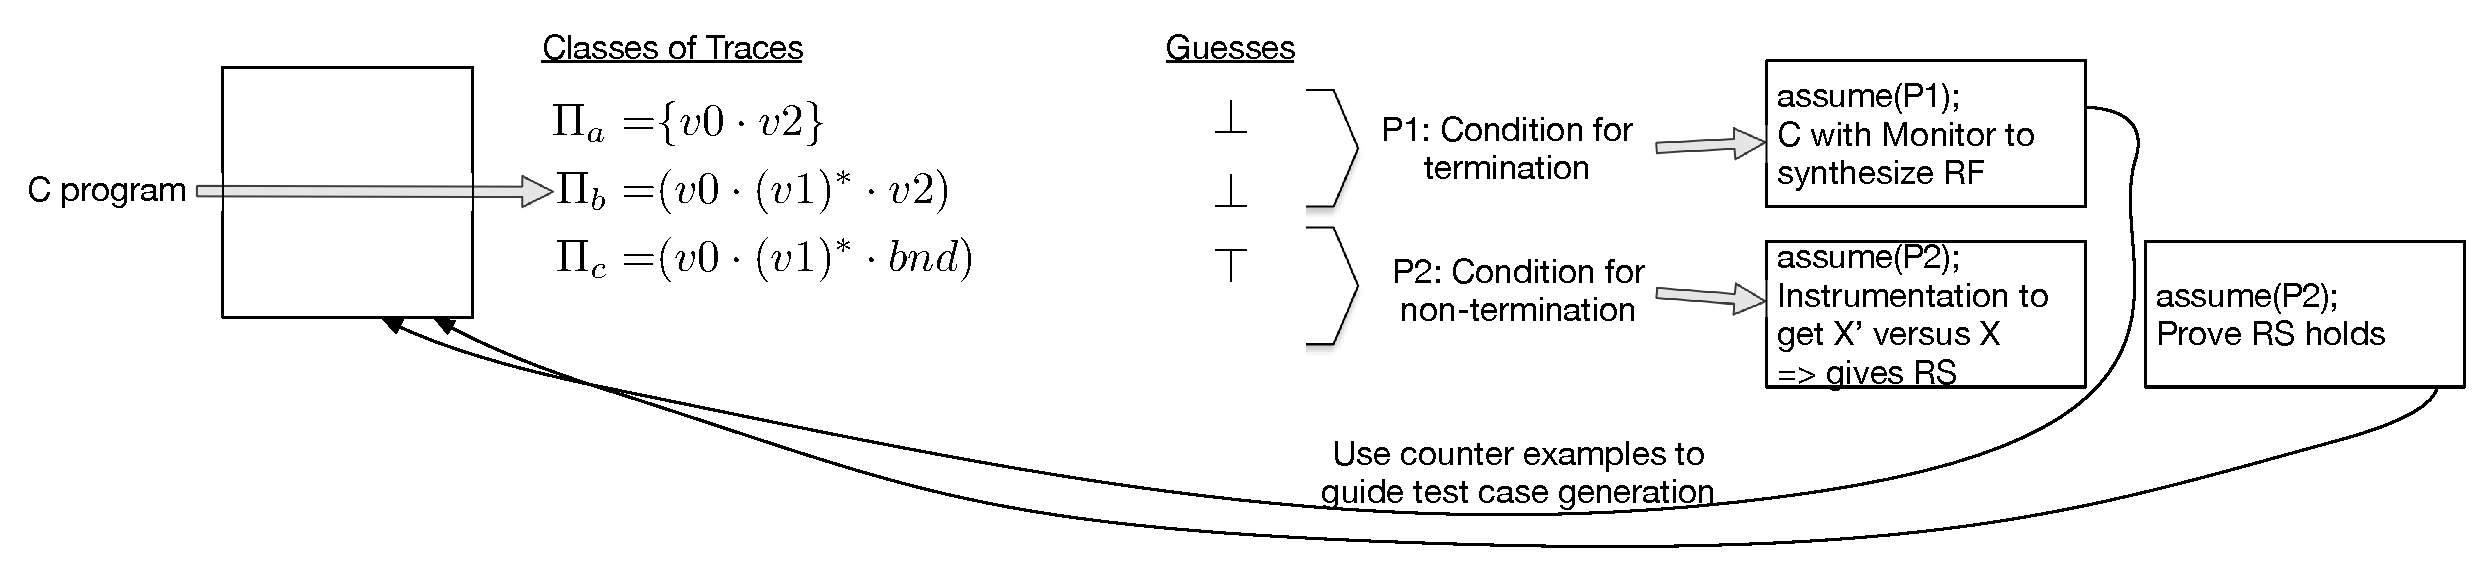
\includegraphics[width=4.5in]{boxes.eps}

\end{center}

\subsection{Expressiveness}

complciated functions like sin, exp, etc.

abstraction

\newcommand\aut{\mathcal{A}}
\newcommand\sem[1]{[\![ #1 ]\!]}

\newcommand\cfarightarrow[1]{\xrightarrow{#1}}
\newcommand\vln{\theta}
\newcommand\Vlns{\Theta}
\newcommand\op{\red{op}}
\newcommand\Ops{\red{Ops}}
\newcommand\states{S}
\newcommand\labels{L}
\newcommand\trans{R}
\newcommand\exect{\textsf{exec}}
\newcommand\rvs{Y}%\overline{r}}
\newcommand\exec[2]{\exect(\vln_{#1},m,\vln_{#2},\rvs)}
\newcommand\execVVM[3]{\exect(\vln_{#1},#3,\vln_{#2},\rvs)}
\newcommand\qv[1]{\langle q_{#1}, \vln_{#1} \rangle}
\newcommand\qtv[1]{\langle q_{#1}, `\vln_{#1} \rangle}

\section{Preliminaries}

\red{cfas or asts?}

\begin{definition}[Control-flow automaton~\cite{Henzinger2002}]
A (deterministic) \emph{control flow automaton} denoted $\aut$, is a
tuple $\aut = \langle Q, q_0, X, s, \cfarightarrow{\,} \rangle$ where $Q$ is a
finite set of control locations and $q_0$ is the initial control location, $X$
is a finite sets of typed variables, $s$ is the statement language (as defined
earlier) and $\cfarightarrow{\,}\subseteq Q \times s \times Q$ is a finite set
of labeled edges.
\end{definition}

\newcommand\run{r}

\paragraph{Valuations and semantics.}
We define a \emph{valuation} of variables 
$\vln : X \rightarrow \mathit{Val}$ to be a mapping from
variable names to values. Let $\Vlns$ be the set of all valuations.
%
The notation $\vln' \in \sem{s}\vln$ means that executing statement $s$, using
the values given in $\vln$, leads to a new
valuation $\vln'$, mapping variables $X$ to new values. Notations $\sem{e}\vln$ and $\sem{b}\vln$ represent side-effect free numeric and boolean valuations, respectively.
%
We assume that for every $\vln,s$, that $\sem{s}\vln$ is computed in finite time.
%
The automaton edges, along with $\sem{s}$, give rise to possible transitions, denoted
$(q,\vln) \cfarightarrow{s} (q',\vln')$ (we omit these rules for lack of space.

A \emph{run} of a CFA is an alternation of automaton states and
valuations: $\run=q_0,\vln_0,q_1,\vln_1,q_2,\dots$
such that $\forall i \geq0.\ (q_i,\vln_i) \cfarightarrow{s} (q_{i+1},\vln_{i+1})$.
%\paragraph{Safety and termination.}
%
We say that CFA $\aut$ can \emph{reach} automaton state $q$ (\emph{safety}) provided that
there exists a run $\run= q_0,\vln_0,q_1,\vln_1,...$ such that there is
some $i \geq 0 $ such that  $q_i=q$.
%
%We say that CFA $\aut$ \emph{terminates} provided that there
%are no infinite runs.
%$\forall q_0,\vln_0,q_1,\vln_1,...\in\Pi(\aut)$ such that there is
%some $i \geq 0 $ such that  $q_i=q$.



%
%
%%% Acknowledgments
%\begin{acks}                            %% acks environment is optional
%                                        %% contents suppressed with 'anonymous'
%  %% Commands \grantsponsor{<sponsorID>}{<name>}{<url>} and
%  %% \grantnum[<url>]{<sponsorID>}{<number>} should be used to
%  %% acknowledge financial support and will be used by metadata
%  %% extraction tools.
%  This material is based upon work supported by the
%  \grantsponsor{GS100000001}{National Science
%    Foundation}{http://dx.doi.org/10.13039/100000001} under Grant
%  No.~\grantnum{GS100000001}{nnnnnnn} and Grant
%  No.~\grantnum{GS100000001}{mmmmmmm}.  Any opinions, findings, and
%  conclusions or recommendations expressed in this material are those
%  of the author and do not necessarily reflect the views of the
%  National Science Foundation.
%\end{acks}


%% Bibliography
%\bibliography{bibfile}


%%% Appendix
%\appendix
%\section{Appendix}
%
%Text of appendix \ldots

\end{document}


